普段ホームページを閲覧する際、ブラウザを開くと思います。アドレスを入力してエンターキーを押すと、あなたが見たいコンテンツが表示されます。この見た目には簡単なユーザの行動には一体何が隠されているのでしょうか?

普通のネットワーク上の操作に対して、システムは実はこのように行なっています:ブラウザそのものはクライアントです。URLを入力する際まずブラウザはDNSサーバにアクセスします。DNSを通してドメインと対応するIPを取得し、IPアドレスからIPに対応したサーバを探しだした後、TCPコネクションの設立を要求します。ブラウザがHTTP Request(リクエスト)パケットを送信し終わると、サーバはリクエストパケットを受け取ってリクエストパケットを処理しはじめます。サーバは自分のサービスをコールし、HTTP Response(レスポンス)パケットを返します。クライアントがサーバからのレスポンスを受け取ると、このレスポンスパケットのbodyを読み出します。すべての内容を受け取ると、このサーバとのTCP接続を切断します。


\begin{figure}[H]
  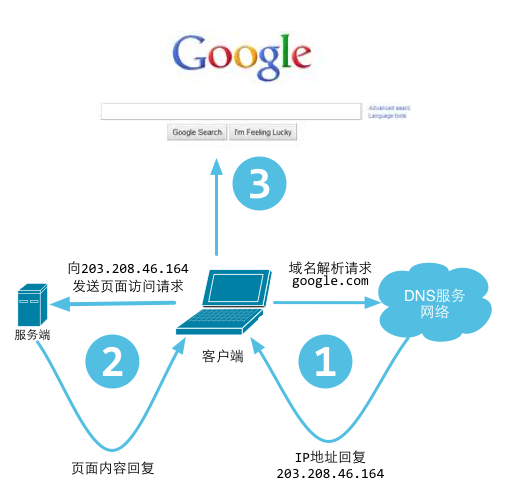
\includegraphics[width=14cm]{3.1.web2.png}
   \label{図3.1}
   \caption{ユーザがWebサーバにアクセスする過程}
\end{figure}


WebサーバはHTTPサーバとも呼ばれます。HTTPプロトコルを通じてクライアントと通信を行います。このクライアントは普通はWebブラウザを指します(実はモバイルクライアントでも内部ではブラウザによって実現されています。)

Webサーバの動作原理は簡単に説明できます:

\begin{itemize}
  \item クライアントがTCP/IPプロトコルによってサーバまでTCP接続を設立します。
  \item クライアントはサーバに対してHTTPプロトコルのリクエストパケットを送信し、サーバのリソースドキュメントを要求します。
  \item サーバはクライアントに対してHTTPプロトコルの応答パケットを送信し、もし要求されたリソースに動的な言語によるコンテンツが含まれている場合、サーバが動的言語のインタープリターエンジンに"動的な内容"の処理をコールさせます。処理によって得られたデータをクライアントに返します。
  \item クライアントとサーバが切断されます。クライアントはHTMLドキュメントを解釈し、クライアントの画面上に図形として結果を表示します。
\end{itemize}


簡単なHTTPタスクはこのように実現されます。見た目にはとても複雑ですが、原理はとても簡単です。気をつけなければならないのは、クライアントとサーバの間の通信は常に接続されているわけではありません。サーバが応答を送信した後クライアントと接続が切断され、次のリクエストを待ち受けます。
